%\graphicspath{ {./sea_vs_blue_f781c5/} }
\graphicspath{ {../figures/} }

\chapter{Seastore performance scaling}

In this Chapter we show the performance scaling of Seastore (build 87d2085) on longer
duration test sets, producing response latency curves. 

\begin{enumerate}
  \item We used a single OSD, running within a single NUMA socket, we only increased the number of reactors as indicated.
  \item We used the balanced OSD algorithm.
  \item We used 32 RBD images, each of 2GB size, four jobs per image. All FIO processes were pinned to the other NUMA socket, so that the OSD processes were not affected by the FIO processes.
  \item We disabled RBD coalescing so the sequential workloads would not be affected by the coalescing algorithm.
\end{enumerate}
%\pagebreak
\section{Random read 4k}

\begin{figure}[!ht]
  \centering
  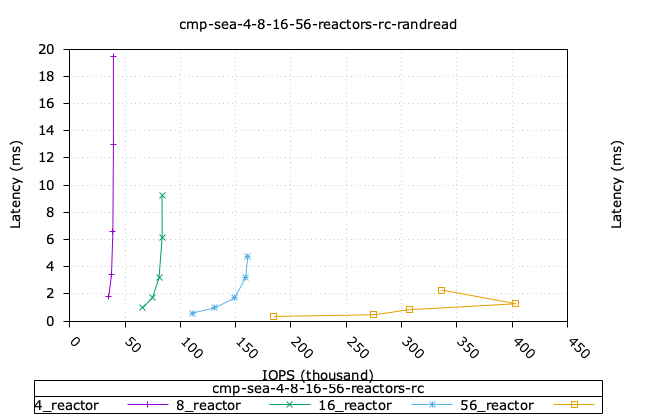
\includegraphics[width=0.9\textwidth]{cmp_sea_4_8_16_56_reactors_rc_randread_iops_vs_lat.png}
  \caption{Response latency curves, IOPs vs. Latency. Each curve is for a different number of reactors, 4, 8, 16 and 56. Each datra point corresponds to an increasing IO depth, from 1 2 4 8 16 24 32 40 52 to 64. If the latency is higher than 1 sec, the data point is not shown. The x-axis is the IOPs, the y-axis is the latency in milliseconds.}
\end{figure}

% utilisation:OSD
% \begin{figure}[h]
%   \centering
%   \begin{minipage}{.5\textwidth}
%   \centering
%     \includegraphics[width=\textwidth]{classic_vs_seastore_1osd_32fio_randread_iops_vs_lat_osd_cpu.png}
%     %\caption{4k random read}
%      %\label{figure:sea_4k_randread}
%   \end{minipage}%
%   \begin{minipage}{.5\textwidth}
%   \centering
%     \includegraphics[width=\textwidth]{classic_vs_seastore_1osd_32fio_randread_iops_vs_lat_osd_mem.png}
%     %\caption{System CPU utilisation}
%     %\label{figure:sea_4k_randwrite}
%   \end{minipage}%
% \end{figure}
%
%In the Tables below we show the performance figures for the workloads above.
% Table showing the figures for this workload
%pagebreak

\section{Random write 4k}

\begin{figure}[ht!]
  \centering
  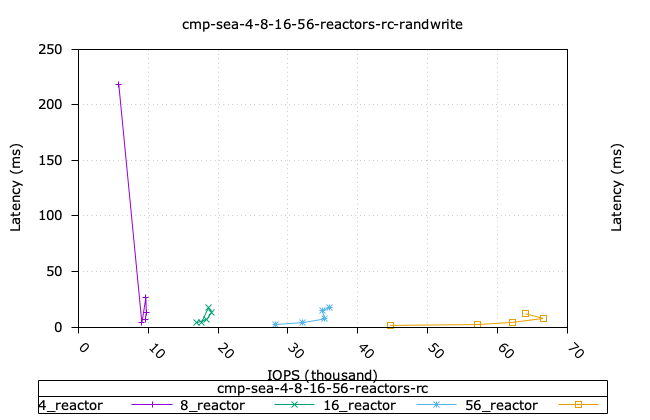
\includegraphics[width=0.9\textwidth]{cmp_sea_4_8_16_56_reactors_rc_randwrite_iops_vs_lat.png}
\end{figure}

% utilisation:OSD
% \begin{figure}[h]
%   \centering
%   \begin{minipage}{.5\textwidth}
%   \centering
%     \includegraphics[width=\textwidth]{classic_vs_seastore_1osd_32fio_randwrite_iops_vs_lat_osd_cpu.png}
%     %\caption{4k random write}
%      %\label{figure:sea_4k_randwrite}
%   \end{minipage}%
%   \begin{minipage}{.5\textwidth}
%   \centering
%     \includegraphics[width=\textwidth]{classic_vs_seastore_1osd_32fio_randwrite_iops_vs_lat_osd_mem.png}
%     %\caption{System CPU utilisation}
%     %\label{figure:sea_4k_randwrite}
%   \end{minipage}%
% \end{figure}
\newpage
\pagebreak

\section{Sequential read 64k}

\begin{figure}[ht]
  \centering
  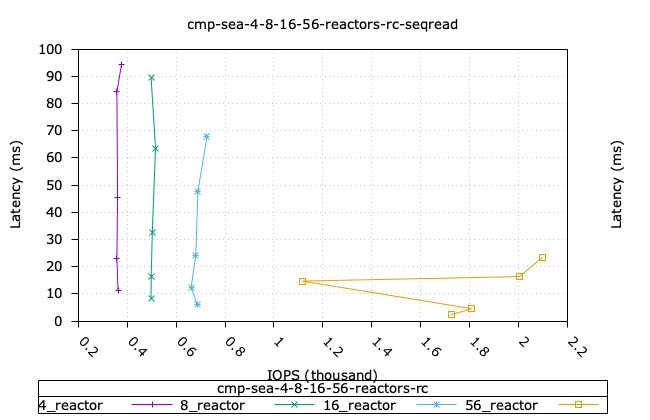
\includegraphics[width=0.9\textwidth]{cmp_sea_4_8_16_56_reactors_rc_seqread_iops_vs_lat.png}
  %\caption{Response latency curves, IOPs vs. Latency}
\end{figure}

% utilisation:OSD
% \begin{figure}[h]
%   \centering
%   \begin{minipage}{.5\textwidth}
%   \centering
%     \includegraphics[width=\textwidth]{classic_vs_seastore_1osd_32fio_seqread_iops_vs_lat_osd_cpu.png}
%     %\caption{4k random write}
%      %\label{figure:sea_4k_seqread}
%   \end{minipage}%
%   \begin{minipage}{.5\textwidth}
%   \centering
%     \includegraphics[width=\textwidth]{classic_vs_seastore_1osd_32fio_seqread_iops_vs_lat_osd_mem.png}
%     %\caption{System CPU utilisation}
%     %\label{figure:sea_4k_seqread}
%   \end{minipage}%
% \end{figure}
%
\newpage
\pagebreak

\section{Sequential write 64k}

\begin{figure}[ht]
  \centering
  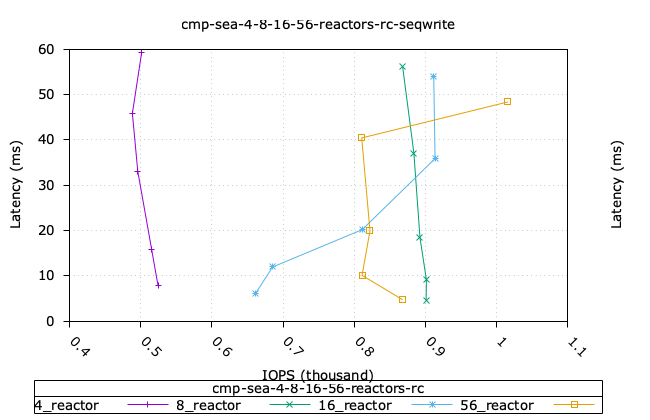
\includegraphics[width=0.9\textwidth]{cmp_sea_4_8_16_56_reactors_rc_seqwrite_iops_vs_lat.png}
  %\caption{Response latency curves, IOPs vs. Latency}
\end{figure}

% % utilisation:OSD
% \begin{figure}[h]
%   \centering
%   \begin{minipage}{.5\textwidth}
%   \centering
%     \includegraphics[width=\textwidth]{classic_vs_seastore_1osd_32fio_seqwrite_iops_vs_lat_osd_cpu.png}
%     %\caption{4k random write}
%      %\label{figure:sea_4k_seqwrite}
%   \end{minipage}%
%   \begin{minipage}{.5\textwidth}
%   \centering
%     \includegraphics[width=\textwidth]{classic_vs_seastore_1osd_32fio_seqwrite_iops_vs_lat_osd_mem.png}
%     %\caption{System CPU utilisation}
%     %\label{figure:sea_4k_seqwrite}
%   \end{minipage}%
% \end{figure}
%
%\newpage


